\subsection{Asynchronous and Parallel Compilation}
\label{sec:framework}
%The need for fast generation of specialized circuits is mostly explained by the the known computer science laws being challegend (dennard, moore, the walls, dark silicon era).
%A recent and emerging solution that allows to follow the pace is OpenSource EDA and its community~\cite{ajayi2019toward}.
%We adopt this approach and build our own open source tool\footnote{\url{https://github.com/Bynaryman/SUF}}.
%Figure~\ref{fig:suf} depicts this framework which enables the generation of many independant design entries from high level description in python to silicon GDS.

The necessity for rapid generation of specialized circuits primarily arises due to the challenges posed to the established laws of computer science, including Dennard scaling, Moore's law, and the emergence of issues like power walls and the dark silicon era.
An advanced and emerging solution that keeps pace is Open Source EDA, supported by its community~\cite{ajayi2019toward}.
In adopting this approach, we build our own open-source tool, accessible online\footnote{\url{https://github.com/Bynaryman/SUF}}.
Figure~\ref{fig:suf} illustrates this framework, which facilitates the creation of multiple independent design entries, transitioning from high-level Python descriptions to silicon GDS outputs.

\begin{figure}[t]
\centering
	%\vspace{-0.5cm}
	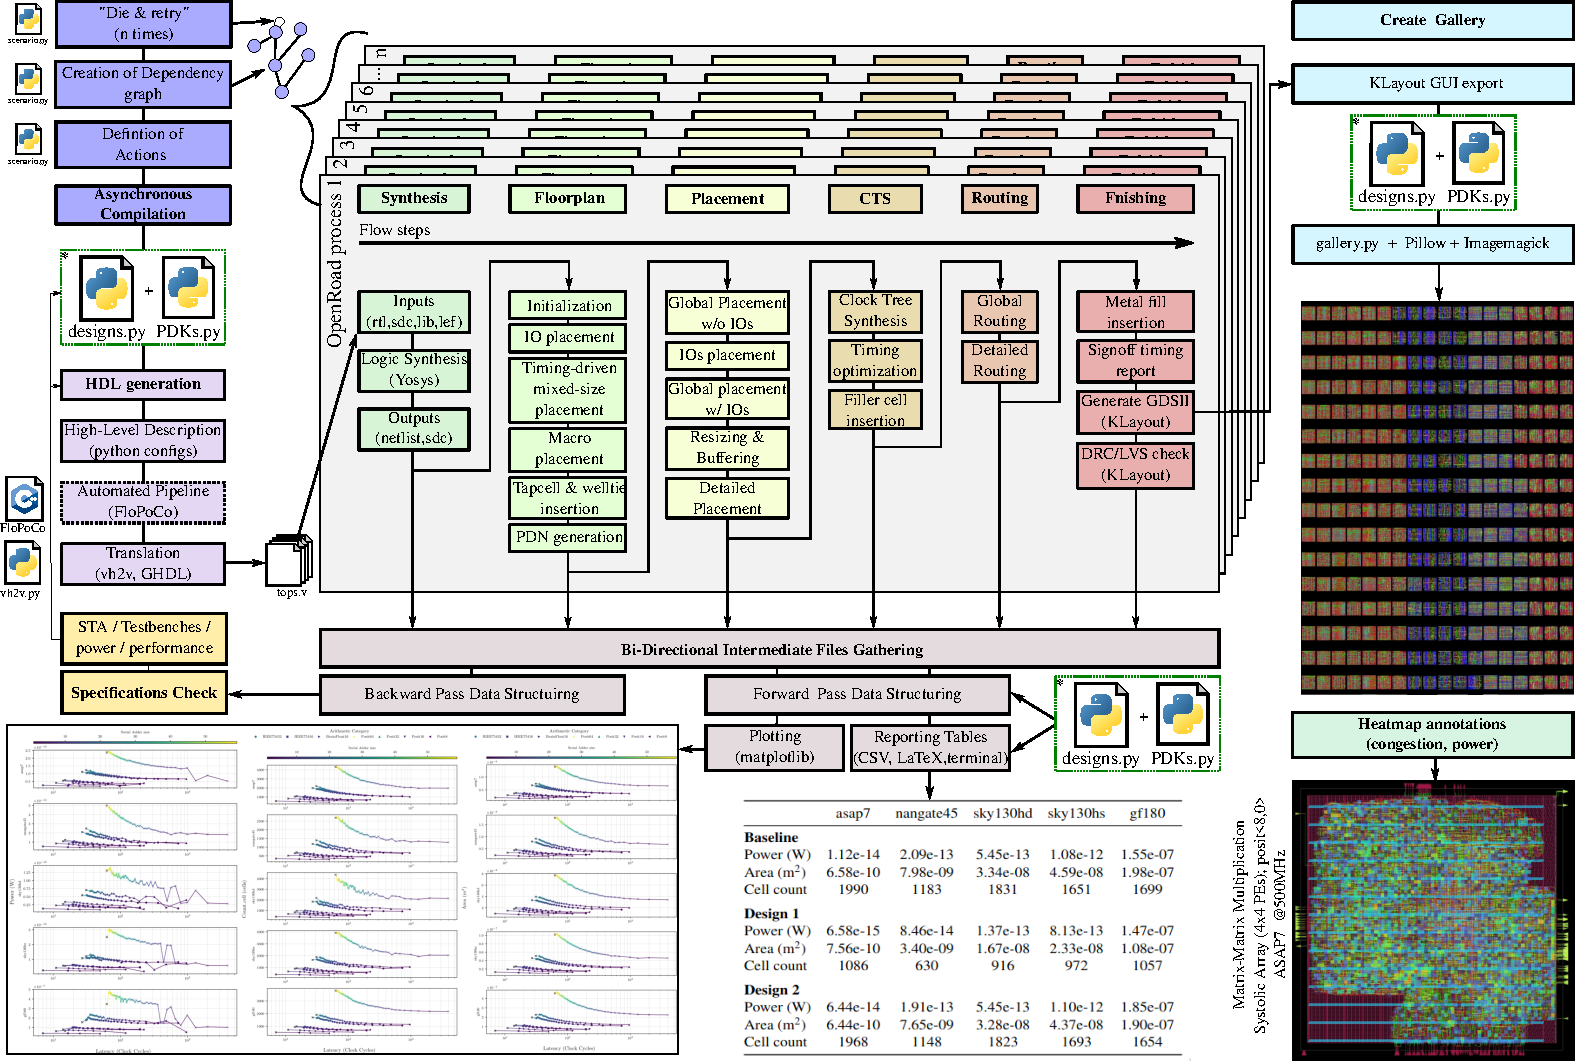
\includegraphics[width=0.9\columnwidth]{./figures/SUF.pdf}
	\vspace{-0.3cm}
	\caption{Schematic Overview SUF: Centralized Management of Asynchronous OpenROAD Forks, Derived from Dependency Task Graphs. This illustration also encapsulates the extended capabilities ranging from Code Generation without manual RTL Writing to Advanced Plotting and Visualization Features.}
	\vspace{-0.3cm}
	\label{fig:suf}
\end{figure}

\begin{figure}[b]
\centering
	\vspace{-0.5cm}
	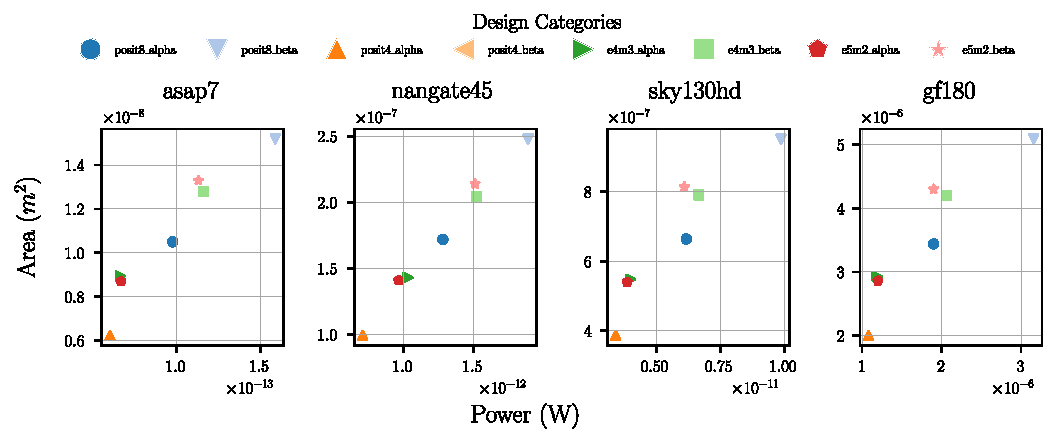
\includegraphics[width=0.9\columnwidth]{./figures/power_vs_area_comparison.pdf}
	\vspace{-0.2cm}
	\caption{Area vs. Power for 28 different MMM units combining diffrent computer format, accumulator sizes, and Process Development Kits.}
	\label{fig:power_vs_area}
\end{figure}

\subsection{Functional and Performance Specifications}
\label{sec:specifications}
We define and assess four computational formats distinguished by their compactness and mathematical attributes (dynamic range and precision).
These include Nvidia's e4m3 and e5m2, and the tapered formats, posit4 (es=0), and posit8(es=2)~\cite{micikevicius_fp8_2022,gustafson_beating_2017}.
Another significant aspect of our work is the proposal of two variations of internal paths for each of these formats.
Internally, we execute the dot product as a fused operation (without rounding) in a fixed accumulator with varying boundaries (bit weights for lsb/msb/ovf).
These variations, named $\alpha$ and $\beta$, are configured as follows: $(\text{ovf}=2,\text{msb}=3,\text{lsb}=-2)$ for an aggregate of 8 bits, and $(\text{ovf}=5,\text{msb}=5,\text{lsb}=-5)$ for the 16-bit model.
The weights distribution of the embedding layers in the Llama-2-7b model dictates these boundaries.
%It is vital to evaluate the trade-offs in the accelerator segment robustly, considering the dynamic range of formats, precision, and sequentialism inherent in MMM algorithms.
All Systolic Arrays of this work are set to $8 \cdot 8=64$ PEs, which ends the defintion of the \textit{Functional} specifications set.

% Performance properties
%We complement this set with \textit{Performance} specifications that span four accross four PDKs, namely GF180, Sky130hd, nangate45, and ASAP7 which are all open (TBD).
%Evaluation of several PDKs allow to verify scalability of designs without the use of manual scaling which are often (make it formal and scientific).
We augment this set with \textit{Performance} specifications across four Process Development Kits (PDKs), specifically GF180, Sky130hd, nangate45, and ASAP7, all of which remain open source.
The assessment of multiple PDKs facilitates the validation of design scalability, obviating the need for often imprecise manual scaling techniques.

%\subsection{Results}
%All the configurations succesfully ``taped out'' in under an hour except for $posit4xbeta$, which makes a total of 28 resulting chips.
%Figure~\ref{fig:all_arrays} depicts in a 2D mesh arranged in arithXaccum VS pdk of the 28 systolic arrays which are their selve 2d meshes.
%Figure~\ref{fig:power_vs_area} presents the performance metrics of the MMM units.
%All beta cost and bigger than alpha, naturally.
%All posits arith cost more compared to their same size coutner part and accum. However, this result needs to be correlated with accuracy (future work).
%e5m2 e4m3 slightly differ and are found in a relatively close clustera stheir HW issimlar.

\subsection{Results}
All configurations successfully ``taped-out'' within an hour, with the exception of posit4$\beta$, culminating in a total of 28 produced chips.
Figure~\ref{fig:all_arrays} illustrates the 28 systolic arrays, each a 2D mesh, arranged across arithmetic units versus PDK dimensions.
Figure~\ref{fig:power_vs_area} details the performance metrics for the MMM units, indicating that beta costs exceed those of alpha, as expected.
Posit arithmetic units incur higher costs relative to their counterparts of equivalent size and accumulation capabilities.
Nonetheless, this observation warrants further investigation into accuracy (designated as future work).
The configurations e5m2 and e4m3 exhibit minor differences and are positioned in closely situated clusters, reflecting their similar hardware characteristics.

\begin{figure}[t]
\centering
	\vspace{-0.5cm}
	\includegraphics[width=0.9\columnwidth]{./figures/systolic_arrays.png}
	%\vspace{-0.5cm}
	\caption{Overview of the GDS layout of the 28 generated MMM units categorized by Arithmetics vs. PDKs. Each layout has a congestion heatmap which helps in the visualization of Processing Elements.}
	\vspace{-0.5cm}
	\label{fig:all_arrays}
\end{figure}

Figure~\ref{fig:focus_on_e4m3} zooms in one of the chip, specifivally the e4m3 arith with beta accumulator for the Sky130 nanometer high density PDK.
The picture allows to see the PEs thanks to routed congestion heatmap.

\begin{figure}[t]
\centering
	%\vspace{-0.5cm}
	\includegraphics[width=0.45\columnwidth]{./figures/SA_8x8_e4m3_rulers_congestion.png}
	%\vspace{-0.5cm}
	\caption{Zoom-in view of the e4m3 beta chip with fine-tunes congestion heatmap allowing to clearly distinguish the $8\times8=64$ PEs.}
	\vspace{-0.5cm}
	\label{fig:focus_on_e4m3}
\end{figure}
